\chapter{Future Research}
\label{chapter:future-research}

\section{Non-Parametric Decision Systems in Non-Euclidian Spaces}

To date, my research has focussed on pushing Gaussian processes (GPs) into the realm of deep learning. I have developed deep convolutional Gaussian processes that mimic the convolutional and layered architectures encountered in many deep learning models \citep{Dutordoir2020convolutional}, Conditional density estimation models which are similar to Variational Auto Encoders (VAEs) \citep{dutordoir2018cde}, and more recently, deep Gaussian processes that have basis functions that are similar to neural network activation functions \citep{dutordoir2021deep}. Through this line of work, I believe that we have showed that (deep) Gaussian processes are an interesting non-parametric alternative to Bayesian neural networks.

In what comes next, I want to separate the different regimes in which neural networks and Gaussian processes operate and thrive. For example, NNs can handle---and in practice require---very large datasets, whereas Gaussian process models are more comfortable in the small data regime. Neural networks, in the presence of large datasets, are extremely good at learning complex latent representations, as evidenced by the latest models in natural language processing and computer vision. Non-parametric Gaussian processes, on the contrary, work best on limited and noisy datasets. Datasets where each datapoint can be very expensive in terms of cost or time to obtain. I believe that this is a setting---in the era of deep learning---that has been under studied and valued, yet of high importance for many scientific or commercial applications.

Many real-world problems can be described as inferring properties of an expensive black-box function $f: \mathcal{X} \rightarrow \mathcal{Y}$, subject to a computational budget of $T$ function evaluations. Typical examples are (global) optimisation, finding a level set (i.e. the set of points in $X \subset \mathcal{X}$ for which $f(x) > C,\forall x \in X$), or finding the shortest path between two nodes in a graph. In the graph example, the black-box function $f$ would return the cost of traversing an edge and query the cost of an edge would be very expensive. Naively applying Dijkstra would require the evaluation of $f$ at every edge and thus potentially grossly exceeding the given budget of $T$ evaluations.


\paragraph{Gaussian processes as surrogate model in non-Euclidian spaces}
We want to place a \emph{surrogate model} between the expensive function $f$ and the algorithm. We model $\tilde{f}$ by a Gaussian process
\begin{equation}
    \tilde{f} \sim \GP
\end{equation}

\begin{enumerate}
    \item Low dimensions
    \item Prior knowledge
    \item Limited, noisy and very expensive data
    \item Non-Euclidian spaces: graphs, meshes, and closed manifolds (e.g. circle).
\end{enumerate}

Basically settings where DNNs are never going to be competitive with GPs - low-dim, very data-efficient, high-cost - not even if someone figures out how to do DNN uncertainty right, due to GP regret guarantees (under reasonable assumptions) matching the best possible regret achievable by any model/decision system.

\paragraph{Related areas}
\begin{enumerate}
    \item Probabilistic numerics [Tubingen Manifesto, Osborne and Henning]. They are less interested in closing the loop and making decisions atop of the models. They usually plot the error bars on the estimator as their final result.
    \item Bayesian optimisation methods. Special case.
\end{enumerate}

\paragraph{Real-world problems}
\begin{itemize}
    \item[Graphs] Social networks. Search for cliques or shortest paths.
    \item[Meshes] Aerospace and civil engineering problems. ``General'' sensor placement.
    \item[Manifold] Sphere. Interesting problem in astrophysics: when a gravitational wave detection is made there's usually a very large uncertainty of its origin so optical telescopes have to sweep the sky looking for the source.
\end{itemize}

\paragraph{Objectives}
\begin{enumerate}
    \item Theory and analysis
    \item Show the excellence of Gaussian processes in this regime
    \item Benchmarks for future methods
\end{enumerate}

\paragraph{Practical}
\begin{enumerate}
    \item Collaborators
    \begin{enumerate}
    \item Alex Terenin (Imperial College London), currently with Marc Deisenroth but starting post-doc at Cambridge.
    \item Willie Neiswanger (Stanford University), with prof. Stefano Ermon.
    \end{enumerate}
    \item We need to find the right problems to solve, which can take time.
\end{enumerate}

% \begin{enumerate}
%     \item Black Box Functions $f: \mathcal{X} \rightarrow \mathcal{Y}$
%     \item We want to estimate a computable property $\mathcal{O}_\mathcal{A}(f)$
%     \item $\mathcal{A}$ is an algorithm $\mathcal{O}_\mathcal{A}(f) = \mathcal{A}(f)$
%     \item Evaluating $f$ is \emph{very} expensive (we can only evaluate it a limited amount of times)
% \end{enumerate}

% \paragraph{Examples}
% \begin{enumerate}
%     \item Optimisation: $\mathcal{A}(f) = \argmax_{x\in\mathcal{X}} f(x)$, which implies $\mathcal{O}_\mathcal{A}(f) = x^*$.
%     \item Sensor Placement (Active Learning): $\mathcal{O}_\mathcal{A}(f) = \argmax_{X \subset \mathcal{X}, |X| = T} \textrm{MI}(f, f(X))$.
%     \item Level sets: $\mathcal{O}_\mathcal{A}(f) = \{X \subset \mathcal{X}: f(x) > C, \forall x \in X\}$.
%     \item Shortest path: $\mathcal{O}_\mathcal{A}(f) = $ shortest path between two nodes in a graph.
% \end{enumerate}



\section{On-going Projects}

\begin{enumerate}
    \item ``Pay Attention to Deep Gaussian Processes''\\
    Transformer Layer Gaussian Processes using an explicit feature representation of the attention operation. The inducing points would play the role of keys in the attention layer.
    \begin{equation*}
        \exp(\vx^\top \vy) = \Phi^\top(\vx) \Phi(\vy)
    \end{equation*}
    % \begin{equation*}
    %     \exp(\vx^\top \vy) = \Phi^\top(\vx) \Phi(\vy)
    % \end{equation*}
    \item Green's Inducing Functions for GPs in Balls
    \begin{enumerate}
        \item Indcing points: adaptivity
        \item Variational Fourier Features: boundary conditions, doesn't scale with dimensionality
        \item Variational Orthogonal Features: 
        \item Spherical Harmonics: restricted in kernel, diagonal Kuu
    \end{enumerate}
    \item VISH-PI: Probabilistic Integration with Variational Inducing Spherical Harmonics, with Michael Osborne and Saad Hamid (student)
\end{enumerate}


% \begin{figure}[htb]
%     \centering % <-- added
% \begin{subfigure}{0.25\textwidth}
%   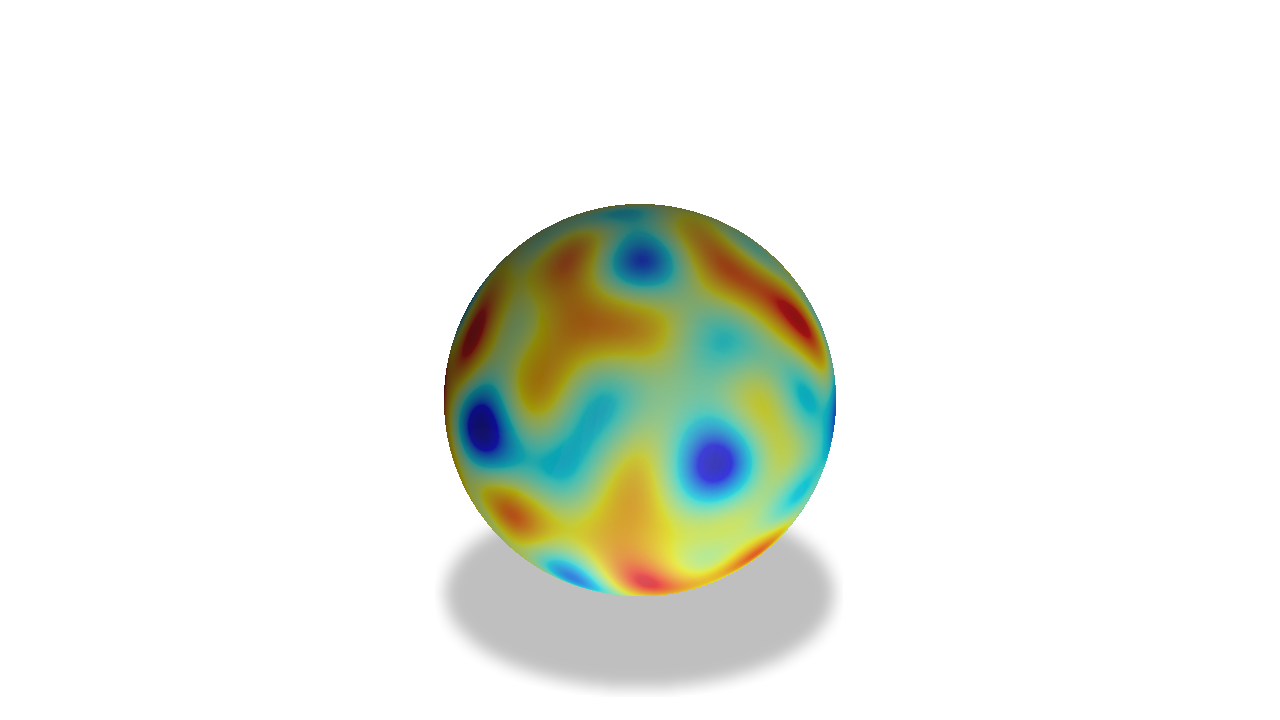
\includegraphics[width=\linewidth]{Chapter5/figures/sphere.png}
% %   \caption{Manifolds}
%   \label{fig:1}
% \end{subfigure}\hfil % <-- added
% \begin{subfigure}{0.25\textwidth}
%   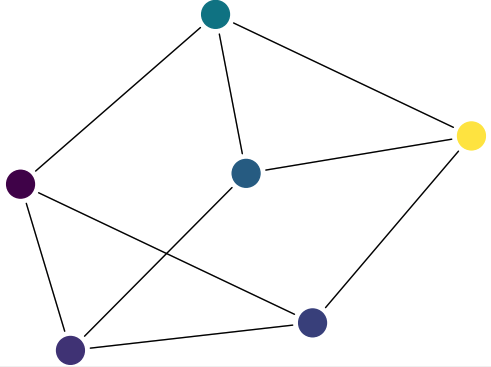
\includegraphics[width=\linewidth]{Chapter5/figures/graph.png}
% %   \caption{Graphs}
%   \label{fig:2}
% \end{subfigure}\hfil % <-- added
% \begin{subfigure}{0.25\textwidth}
%   \includegraphics[width=\linewidth]{Chapter5/figures/BunnyWire.png}
% %   \caption{Meshes}
%   \label{fig:3}
% \end{subfigure}

% \medskip
% \begin{subfigure}{0.25\textwidth}
%   \includegraphics[width=\linewidth]{Chapter5/figures/cosmos.png}
% %   \caption{Cosmos}
%   \label{fig:4}
% \end{subfigure}\hfil % <-- added
% \begin{subfigure}{0.25\textwidth}
%   \includegraphics[width=\linewidth]{Chapter5/figures/social_network.png}
% %   \caption{image5}
%   \label{fig:5}
% \end{subfigure}\hfil % <-- added
% \begin{subfigure}{0.25\textwidth}
%   \includegraphics[width=\linewidth]{Chapter5/figures/mesh_engine.png}
% %   \caption{image6}
%   \label{fig:6}
% \end{subfigure}
% \caption{Domains (top) and applications (bottom)}
% \label{fig:images}
% \end{figure}
